\chapter{Risultati sperimentali}
\label{cap:risultati}

Al fine di valutare il comportamento del sistema nelle condizioni operative previste, sono stati condotti una serie di test sperimentali inviando alla Board A, tramite uno script Python, immagini di veicoli con targa visibile, sia di nazionalità italiana che straniera, così da verificare la generalizzazione della pipeline su formati differenti. È stato inoltre incluso un caso negativo, ovvero un'immagine priva di veicoli, per osservare la risposta del sistema in assenza di una targa rilevabile. Per ciascun test vengono riportati l'immagine di input e la stringa riconosciuta restituita dalla Board B. Oltre ai risultati qualitativi del riconoscimento, vengono discussi i dati relativi all'occupazione della memoria (Flash e RAM) dei firmware caricati sulle due schede, nonché i tempi di computazione end-to-end misurati sull'intera pipeline, dall'invio e ricezione dell'immagine alla restituzione della targa riconosciuta.

\section{Configurazione del test}
\label{sec:test-setup}

Lo script Python di test (\texttt{plate\_recognition.py}) carica una singola immagine da disco, la pre-elabora portandola a $192\times192$ pixel in scala di grigi, e la invia alla Board A in un frame \texttt{TYPE\_GRAY}. Il tempo end-to-end è misurato sul PC tra l'invio del frame e la ricezione della risposta finale, comprendendo dunque tutti i trasferimenti UART, le due inferenze e l'overhead di sincronizzazione tra le board. La temporizzazione è effettuata con \texttt{time.perf\_counter()} di Python, che garantisce risoluzione al microsecondo.

Le immagini di test sono state selezionate per coprire condizioni eterogenee: targhe inquadrate frontalmente e di lato, con diversi livelli di illuminazione. Il dataset comprende un'immagine di paesaggio senza alcun veicolo, deliberatamente inclusa per verificare il corretto comportamento del sistema in assenza di targhe (caso che dovrebbe attivare la risposta \texttt{TYPE\_NONE}).

\section{Occupazione di memoria}
\label{sec:memoria-occupazione}

Al termine della build di entrambi i firmware, il sistema di compilazione di Zephyr riporta l'occupazione delle sezioni di memoria nella tabella di sintesi del linker. La Tabella~\ref{tab:footprint} riassume i valori misurati, si tenga conto che per entrambe le board la memoria Flash totale è di 1~MB e la memoria RAM totale di 512~KB.

\begin{table}[H]
    \centering
    \begin{tabular}{lrrrr}
        \toprule
        \textbf{Board} & \textbf{Flash usato} & \textbf{\% Flash} & \textbf{RAM usata} & \textbf{\% RAM} \\
        \midrule
        Board A (detection) & 907{,}16~KB & 88{,}59~\% & 502{,}00~KB & 98{,}05~\% \\
        Board B (OCR)       & 812{,}23~KB & 79{,}32~\% & 384{,}63~KB & 75{,}12~\% \\
        \bottomrule
    \end{tabular}
    \caption{Occupazione di Flash e RAM dei due firmware}
    \label{tab:footprint}
\end{table}

\begin{figure}[H]
    \centering
    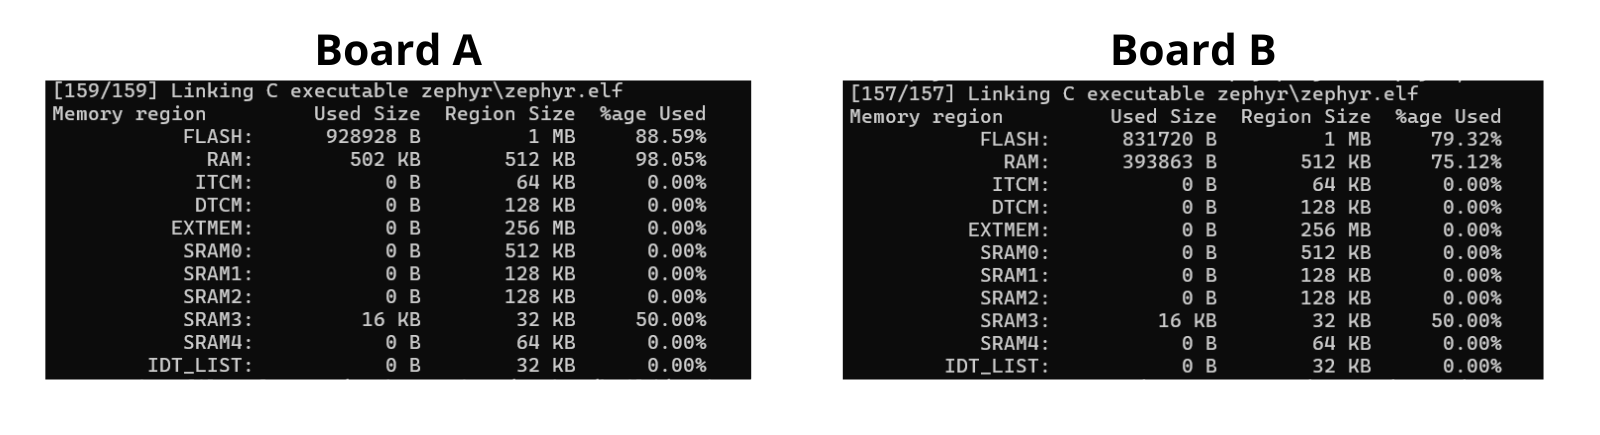
\includegraphics[width=0.95\textwidth]{images/occupazione_memoria_board.png}
    \caption{Output del linker Zephyr al termine della build dei due firmware}
    \label{fig:occupazione_memoria}
\end{figure}

Il dato più significativo è la quasi saturazione della RAM su Board A, a $98{,}05\,\%$ della capacità disponibile (502 KB su 512 KB, con appena 10 KB di margine residuo). Questo risultato non è casuale: l'occupazione è dominata dal solo buffer delle \textit{activation} della rete YOLO, che richiede 410\,112 byte ($\approx400$~KB). A questo si sommano l'\texttt{io\_buf} da 36\,864 byte, il \texttt{crop\_buf} da 8\,196 byte, i due ring buffer e il footprint statico del runtime Zephyr. Le ottimizzazioni descritte nei capitoli precedenti, in particolare l'uso della \texttt{union} per condividere lo stesso spazio tra l'immagine ricevuta e il tensore di input quantizzato, sono state necessarie per restare entro il budget disponibile. Sulla Board B la situazione è più rilassata: l'\textit{activation buffer} del CCT-XS richiede 296\,212 byte ($\approx289$~KB), inferiore di oltre 100~KB rispetto a quello di YOLO, e questo lascia un margine confortevole per il resto delle strutture dati. Anche l'occupazione di Flash è minore, perché il modello CCT-XS pesa circa 500~KB contro i 617~KB del modello YOLO.

Si può notare nella Figura \ref{fig:occupazione_memoria} che le regioni di memoria aggiuntive presenti sul microcontrollore, come ITCM, DTCM, SRAM0-4 ed EXTMEM, risultano inutilizzate in quanto il loro impiego richiederebbe un mapping esplicito nel linker script di Zephyr e un posizionamento manuale dei singoli buffer tramite attributi di sezione. Inoltre, strutture dati che per loro natura devono essere contigue in memoria,come i buffer di attivazione della rete neurale, non possono essere suddivise tra regioni fisicamente separate, rendendo di fatto impraticabile una distribuzione trasparente dei dati su più banchi. Per questi motivi, tutto il firmware è stato allocato nella regione RAM principale, che costituisce l'unica area di memoria gestita automaticamente da Zephyr.

\section{Risultati di riconoscimento}
\label{sec:risultati-riconoscimento}

Il sistema è in grado di riconoscere correttamente targhe italiane standard (formato $LL\,DDD\,LL$) ma anche straniere, a patto che siano presenti nel file di configurazione \texttt{.yaml} del relativo modello OCR presente nella repository utilizzata \cite{ankandrew_2024_fastplateocr}. \\
Sono stati condotti dei test utilizzando immagini di veicoli con targhe di nazionalità italiana, svizzera e tedesca, che differiscono tra loro per struttura, font e numero di caratteri. Di seguito, nelle Figure \ref{fig:riconoscimento_targhe_italiane} e \ref{fig:riconoscimento_targhe_straniere}, vengono riportati alcuni risultati rappresentativi: per ciascun caso è mostrata l'immagine originale che viene trasformata e inviata tramite lo script Python e il risultato finale di riconoscimento sotto forma di output nel terminale.

\begin{figure}[H]
    \centering
    % Prima riga
    \begin{subfigure}[t]{0.4\textwidth}
        \centering
        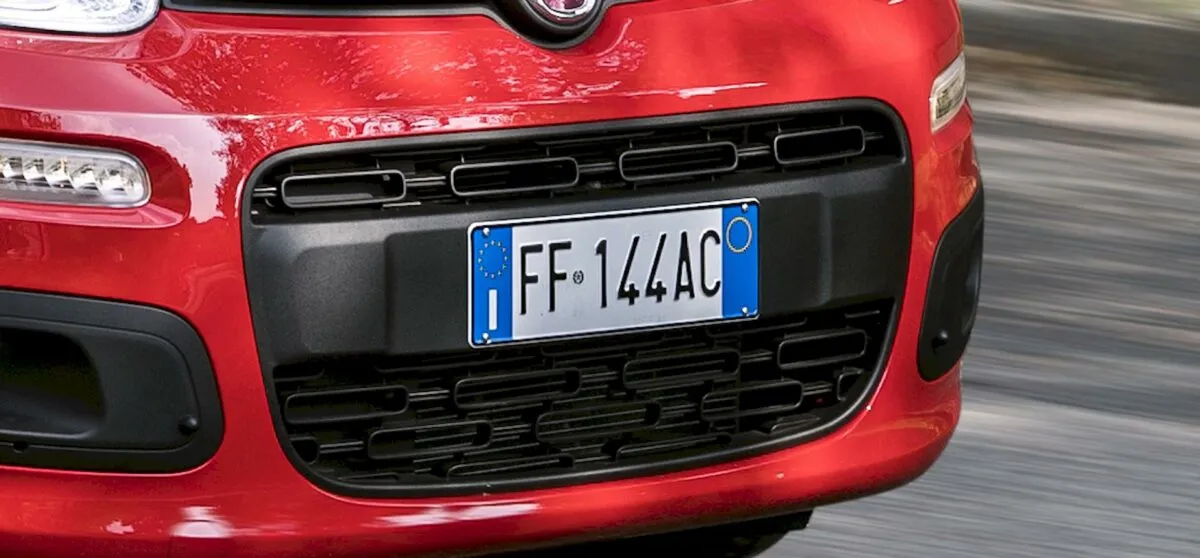
\includegraphics[width=\textwidth]{images/plate_25.png}
        \caption{Immagine originale}
        \label{fig:targa_originale_1}
    \end{subfigure}
    \hfill
    \begin{subfigure}[t]{0.59\textwidth}
        \centering
        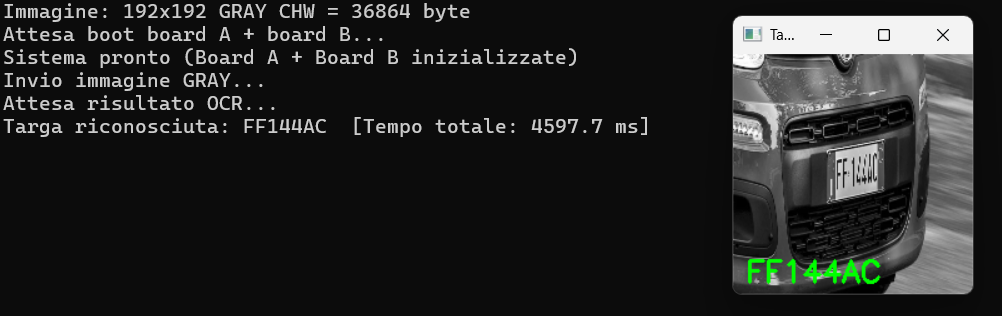
\includegraphics[width=\textwidth]{images/targa_italiana_riconosciuta.png}
        \caption{Output di riconoscimento della targa}
        \label{fig:output_targa_1}
    \end{subfigure}

    \vspace{0.5cm} % Spazio verticale tra le due righe

    % Seconda riga
    \begin{subfigure}[t]{0.4\textwidth} 
    \centering
    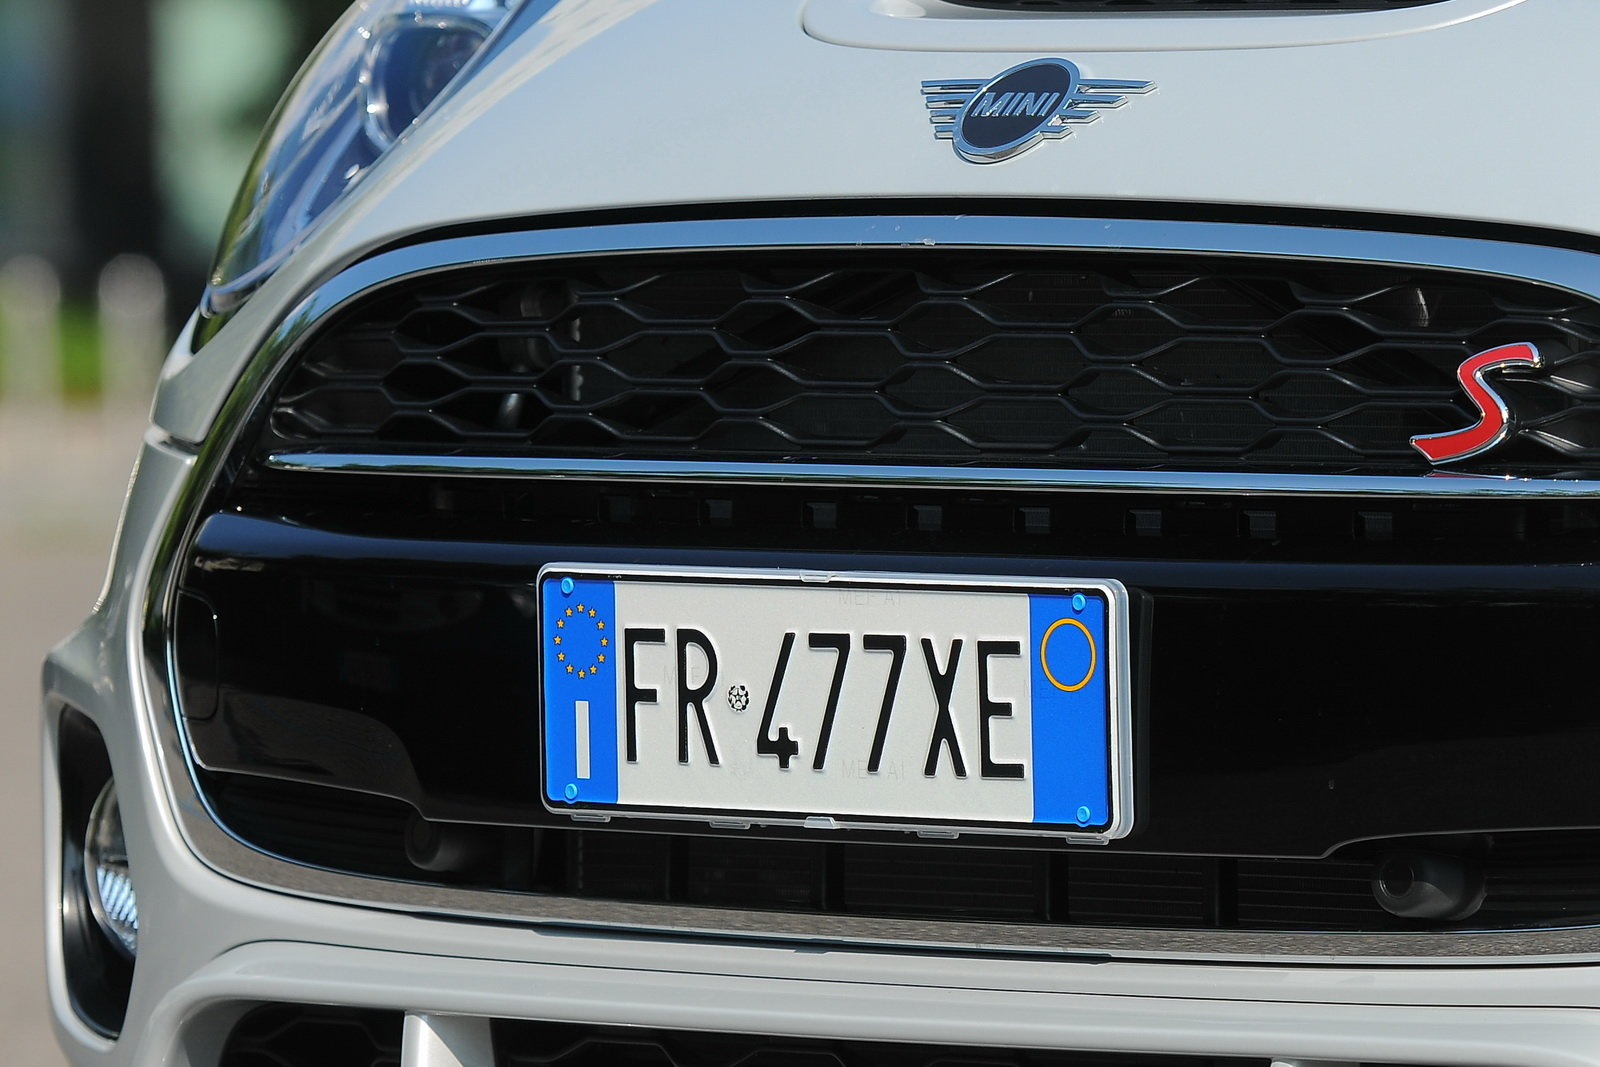
\includegraphics[
        width=\textwidth,
        trim=0 2cm 0 8cm,
        clip
    ]{images/plate_23.jpg}
    \caption{Immagine originale}
    \label{fig:targa_originale_2}
    \end{subfigure}
    \hfill
    \begin{subfigure}[t]{0.59\textwidth}
        \centering
        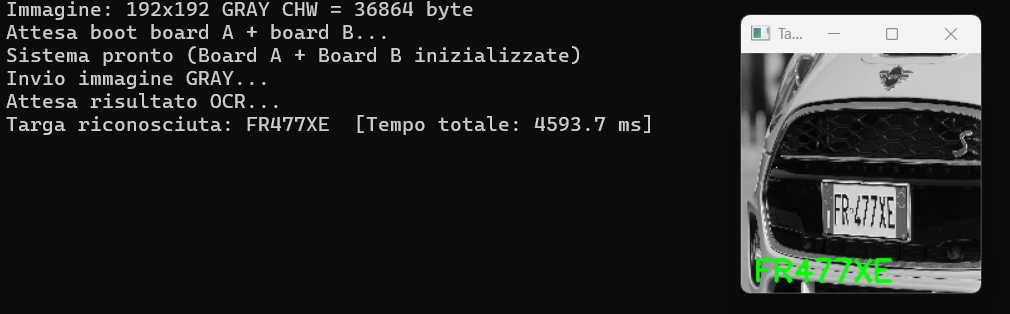
\includegraphics[width=\textwidth]{images/targa_italiana_riconosciuta_2.png}
        \caption{Output di riconoscimento della targa}
        \label{fig:output_targa_2}
    \end{subfigure}

    \caption{Esempi di riconoscimento corretto di targhe italiane}
    \label{fig:riconoscimento_targhe_italiane}
\end{figure}

\begin{figure}[H]
    \centering
    % Prima riga
    \begin{subfigure}[t]{0.4\textwidth}
        \centering
        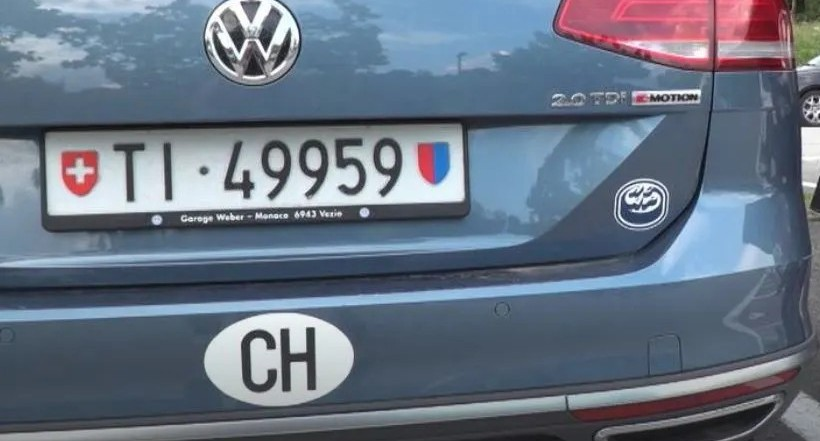
\includegraphics[width=\textwidth,
        trim=0 0 0 1.8cm,
        clip]{images/plate_21.jpg}
        \caption{Immagine originale}
        \label{fig:targa_originale_3}
    \end{subfigure}
    \hfill
    \begin{subfigure}[t]{0.59\textwidth}
        \centering
        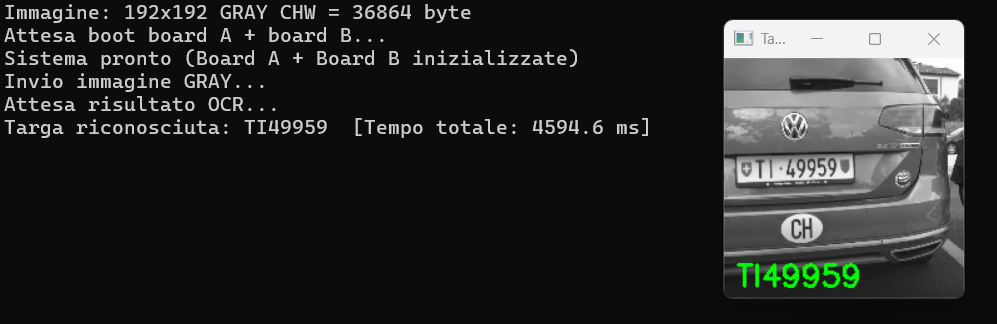
\includegraphics[width=\textwidth]{images/targa_svizzera_riconosciuta.png}
        \caption{Output di riconoscimento della targa}
        \label{fig:output_targa_3}
    \end{subfigure}

    \vspace{0.5cm} % Spazio verticale tra le due righe

    % Seconda riga
    \begin{subfigure}[t]{0.4\textwidth}
        \centering
        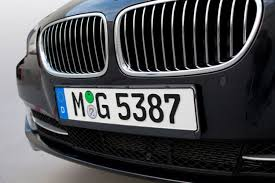
\includegraphics[width=\textwidth,
        trim=0 0 0 2cm,
        clip]{images/plate_14.jpg}
        \caption{Immagine originale}
        \label{fig:targa_originale_4}
    \end{subfigure}
    \hfill
    \begin{subfigure}[t]{0.59\textwidth}
        \centering
        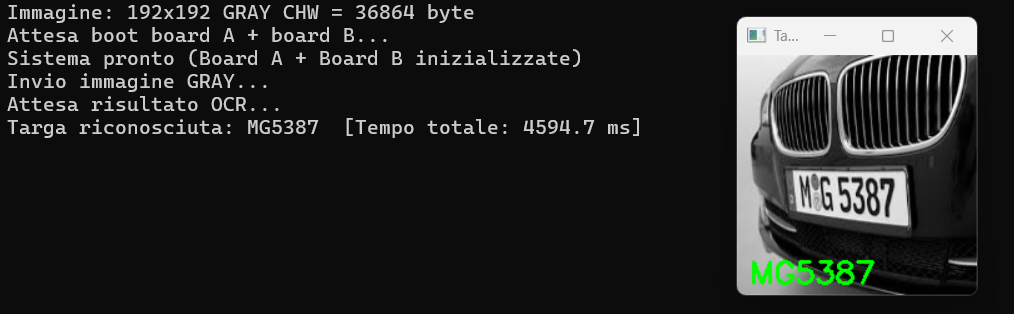
\includegraphics[width=\textwidth]{images/targa_tedesca_riconosciuta.png}
        \caption{Output di riconoscimento della targa}
        \label{fig:output_targa_4}
    \end{subfigure}

    \caption{Esempi di riconoscimento corretto di targe straniere (Svizzera e Germania)}
    \label{fig:riconoscimento_targhe_straniere}
\end{figure}

\subsection{Tempo end-to-end}
\label{sec:tempo-eed}

I tempi end-to-end misurati sulle quattro immagini precedente con detection riuscita sono riportati in Tabella~\ref{tab:tempi}. Il valore medio è di $4595{,}17$~ms con deviazione standard di $1{,}74$~ms: la latenza del sistema è dunque marcatamente deterministica, segno che l'esecuzione su Cortex-M7 senza task concorrenti non subisce variazioni di rilievo da un'esecuzione all'altra.

\begin{table}[H]
    \centering
    
    \begin{tabular}{lcc}
        \toprule
        \textbf{\#} & \textbf{Targa riconosciuta} & \textbf{Tempo (ms)} \\
        \midrule
        1 & FF144AC                   & 4597{,}7 \\
        2 & FR477XE                   & 4593{,}7 \\
        3 & TI49959                   & 4594{,}6 \\
        4 & MG5387                    & 4594{,}7 \\
        \midrule
        \multicolumn{2}{l}{\textit{Media}}   & $\mathbf{4595{,}17}$ \\
        \multicolumn{2}{l}{\textit{Std.dev.}} & $\mathbf{1{,}74}$ \\
        \bottomrule
    \end{tabular}
    \caption{Tempi end-to-end misurati su quattro immagini con detection riuscita}
    \label{tab:tempi}
\end{table}

\subsection{Analisi del bottleneck}
\label{sec:bottleneck}

La latenza di circa $4{,}6$~secondi è eccessiva per applicazioni in tempo reale, ed è utile capirne la composizione. Un calcolo a priori mostra che la sola trasmissione seriale è già il fattore dominante:

\begin{itemize}
    \item Il canale UART a 115\,200~baud con codifica 8N1 (10 bit per byte trasmesso, considerando bit di start e stop) sostiene un throughput utile di $11\,520$~byte/s.
    \item L'immagine $192\times192$ grayscale è di $36\,864$ byte, dunque la trasmissione PC~$\rightarrow$~A richiede $\approx3{,}20$~s.
    \item Il crop $128\times64$ è di $8\,192$ byte, dunque A~$\rightarrow$~B richiede $\approx0{,}71$~s.
\end{itemize}

La somma dei due trasferimenti seriali ammonta a circa 3,91 s, corrispondenti a circa l'85\% del tempo end-to-end osservato, evidenziando come il \textbf{collo di bottiglia principale} del sistema sia la comunicazione UART e non l'elaborazione neurale. I restanti $\approx680$~ms includono il tempo necessario per le due inferenze, insieme al post-processing, che comprende la Non-Maximum Suppression, la costruzione del crop, l'espansione da grayscale a RGB, la decodifica finale della targa e il sovraccarico legato alla sincronizzazione del protocollo.\\
È importante sottolineare che questo risultato va interpretato nel contesto sperimentale adottato: in una configurazione reale, il trasferimento iniziale dell'immagine dal PC alla Board A verrebbe infatti eliminato, sostituendo il PC con una videocamera direttamente collegata alla scheda. In tale scenario, la latenza complessiva si ridurrebbe sensibilmente, restando sostanzialmente limitata ai tempi di inferenza e post-processing sulla Board A e al trasferimento del crop verso la Board B, pari a circa 710 ms. Anche quest'ultimo contributo, tuttavia, può essere ulteriormente ridotto con interventi mirati, ad esempio aumentando il baud rate della comunicazione inter-board o adottando un'interfaccia più veloce come SPI.\\
Nel complesso, questi risultati mostrano che l'architettura distribuita proposta è solida e adatta a un impiego embedded autonomo e che i principali margini di miglioramento riguardano soprattutto il canale di comunicazione, più che la capacità di inferenza delle due schede.

\begin{boxH}
\textbf{In sintesi.} A 115\,200~baud, la sola trasmissione dei dati attraverso le UART occupa $\sim$3{,}9~s su 4{,}6~s di latenza totale. Le due inferenze, anche se impegnative per un Cortex-M7 senza acceleratore neurale, occupano nell'insieme meno del $15\,\%$ del tempo end-to-end, il che è un risultato ottimo.
\end{boxH}

\section{Validazione sul caso negativo}
Al fine di valutare la robustezza del sistema in assenza di un oggetto di interesse, è stato condotto un test inviando alla Board A un'immagine priva di veicoli e quindi priva di targhe rilevabili. L'obiettivo è verificare che la pipeline gestisca correttamente questo caso, rispondendo in modo appropriato senza produrre riconoscimenti errati o comportamenti inattesi. Il risultato di tale test si può osservare in Figura \ref{fig:riconoscimento_caso_negativo}.

\begin{figure}[H]
    \centering
    % Prima riga
    \begin{subfigure}[t]{0.34\textwidth}
        \centering
        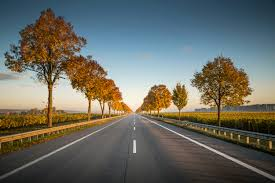
\includegraphics[width=\textwidth,
        trim=0 1cm 0 1.5cm,
        clip]{images/plate_26.jpg}
        \caption{Immagine originale}
        \label{fig:targa_originale_5}
    \end{subfigure}
    \hfill
    \begin{subfigure}[t]{0.65\textwidth}
        \centering
        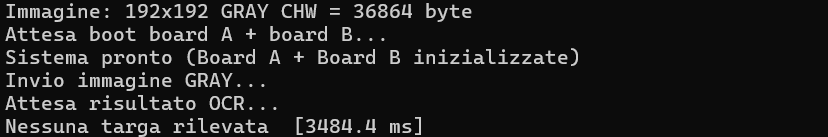
\includegraphics[width=\textwidth,
        trim=0 0 4cm 0,
        clip]{images/nessuna_targa.png}
        \caption{Output di riconoscimento della targa}
        \label{fig:output_targa_5}
    \end{subfigure}
    \caption{Esempio di riconoscimento del caso negativo: assenza di targhe}
    \label{fig:riconoscimento_caso_negativo}
\end{figure}
Il sistema, correttamente, produce una risposta \texttt{TYPE\_NONE} per cui nel log viene mostrata la frase "Nessuna targa rilevata". È interessante notare che il \textbf{tempo di risposta} è $\mathbf{3\,484{,}4}$~\textbf{ms}. Questo tempo è di circa $1\,100$~ms inferiore al caso con detection riuscita, e la differenza è esattamente quella attesa: viene a mancare il trasferimento del crop a Board~B (0{,}71~s) più la sua inferenza CCT e il viaggio di ritorno della stringa. Il caso è interessante perché conferma che il flusso di errori del protocollo funziona: in assenza di anchor sopra soglia, Board~A non tenta di forzare una predizione ma comunica esplicitamente al PC l'esito negativo.



\section{Analisi degli errori di riconoscimento}
\label{sec:errori}

In questa sezione vengono presentati alcuni casi in cui il sistema ha commesso errori di riconoscimento, al fine di analizzarne il comportamento in condizioni non ideali. I risultati riportati consentono di evidenziare le principali criticità emerse durante le prove sperimentali e di discutere le possibili cause degli errori osservati. Nella Figura \ref{fig:errori_riconoscimento_targhe_italiane} si possono notare due casi in cui è avvenuto un errore di riconoscimento delle targhe.

\begin{figure}[H]
    \centering
    % Prima riga
    \begin{subfigure}[t]{0.35\textwidth}
        \centering
        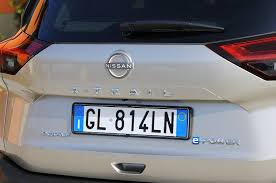
\includegraphics[width=\textwidth,
        trim=0 0 0 1cm,
        clip]{images/plate_2.jpg}
        \caption{Immagine originale}
        \label{fig:targa_originale_6}
    \end{subfigure}
    \hfill
    \begin{subfigure}[t]{0.64\textwidth}
        \centering
        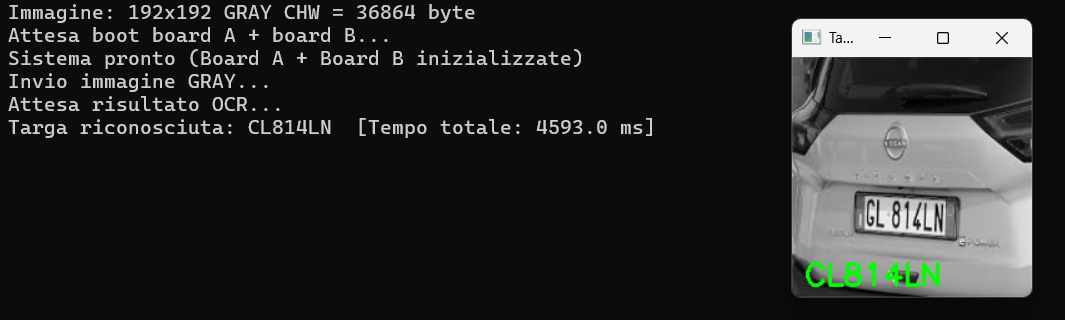
\includegraphics[width=\textwidth]{images/targa_italiana_errore2.png}
        \caption{Output di riconoscimento della targa}
        \label{fig:output_targa_6}
    \end{subfigure}

    \vspace{0.5cm} % Spazio verticale tra le due righe

    % Seconda riga
    \begin{subfigure}[t]{0.35\textwidth}
        \centering
        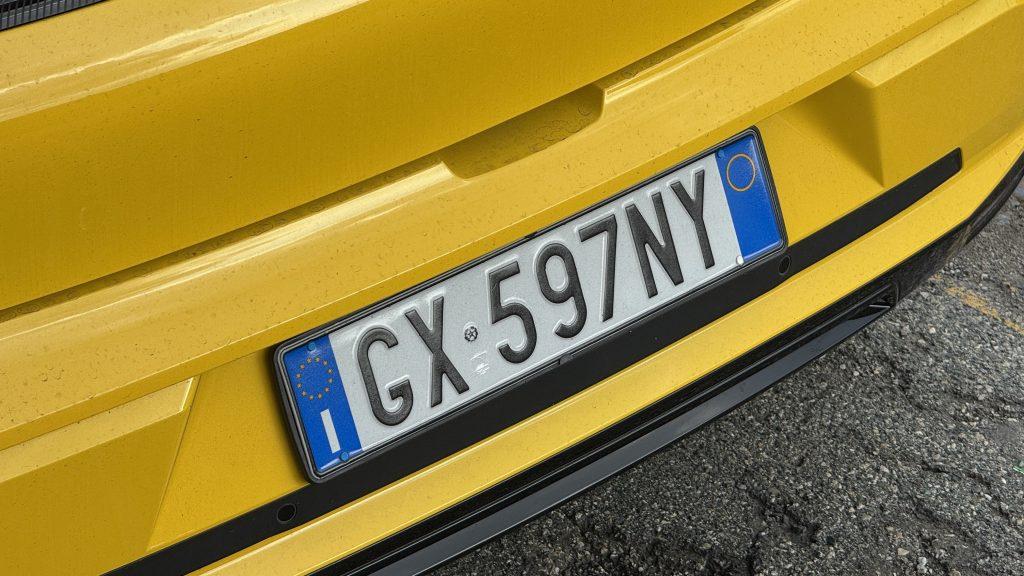
\includegraphics[width=\textwidth]{images/plate_4.jpg}
        \caption{Immagine originale}
        \label{fig:targa_originale_7}
    \end{subfigure}
    \hfill
    \begin{subfigure}[t]{0.64\textwidth}
        \centering
        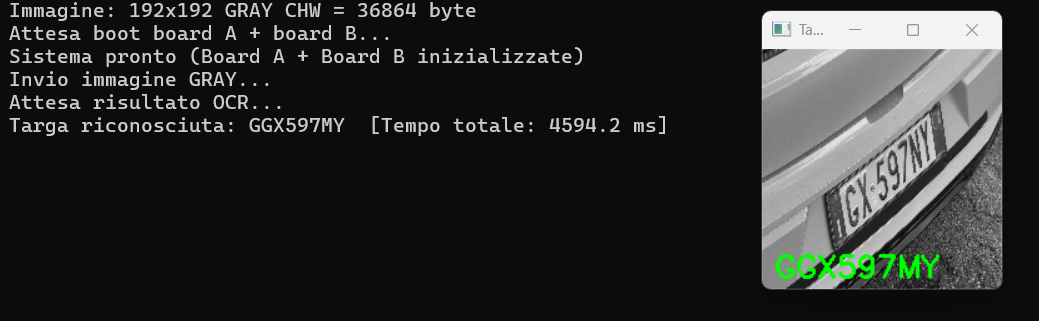
\includegraphics[width=\textwidth]{images/targa_italiana_errore1.png}
        \caption{Output di riconoscimento della targa}
        \label{fig:output_targa_7}
    \end{subfigure}

    \caption{Esempi di errori di riconoscimento in targhe italiane}
    \label{fig:errori_riconoscimento_targhe_italiane}
\end{figure}

Gli errori principali commessi dal sistema sono riconducibili ai seguenti:

\begin{itemize}
    \item \textbf{Slot duplicati}: nella Figura \ref{fig:output_targa_7}, la targa originale \texttt{GX597NY} viene letta come \texttt{GGX597MY}, con il primo carattere ripetuto. Si tratta di un'incertezza sull'allineamento spaziale dei caratteri all'interno della targa: il primo carattere si trova in una posizione che la rete fatica a discretizzare correttamente in uno dei 9 slot disponibili, e finisce per attivare due slot adiacenti. La causa di ciò è che, nell'immagine originale, la targa risulta inclinata e non perfettamente allineata orizzontalmente, rendendo più difficile la corretta segmentazione dei caratteri.
    \item \textbf{Confusione tra caratteri visivamente simili}: in entrambe le Figure (\ref{fig:output_targa_6} e \ref{fig:output_targa_7}) si nota questo errore. Nel primo caso, la targa originale \texttt{GL814LN} viene letta come \texttt{CL814LN}, con la \texttt{G} iniziale scambiata per \texttt{C}. Nel secondo caso, invece, la targa \texttt{GX597NY} viene riconosciuta come \texttt{GGX597MY}, mostrando sia la duplicazione del carattere iniziale (già discusso) sia l'errore sulla parte finale della stringa. Questi risultati evidenziano una limitazione tipica dei modelli OCR operanti a bassa risoluzione (in questo caso $128\times64$), dove caratteri visivamente simili possono essere confusi con maggiore facilità. La criticità può essere ulteriormente accentuata dal fatto che, quando il bounding box rilevato risulta più piccolo della risoluzione richiesta dalla rete OCR, viene applicato un upscaling dell'immagine: tale operazione, pur necessaria per adattare l'input al modello, può introdurre artefatti o amplificare differenze minime tra caratteri simili, contribuendo all'errore di classificazione.

\end{itemize}

Gli errori osservati dipendono soprattutto dalla \textbf{rete OCR pre-addestrata}, mentre YOLO individua in genere bounding box coerenti. Le criticità emergono nella lettura dei caratteri, specialmente con input difficili o a bassa risoluzione. In questi casi l'OCR può confondere simboli simili. Un possibile miglioramento consiste nel fine-tuning su un dataset più specifico.
